\documentclass[a4paper]{article}
\usepackage[swedish, english]{babel}
\usepackage[T1]{fontenc}
\usepackage[sectionbib, round, authoryear, longnamesfirst]{natbib}
\renewcommand{\rmdefault}{pad}
\usepackage{graphicx}
\usepackage{tabularx}
\usepackage[a4paper]{geometry}
\usepackage{url}
\usepackage{amsmath}
\usepackage{setspace}
\onehalfspacing
\numberwithin{equation}{section}
\usepackage{lscape}
\usepackage{makeidx}
\makeindex

% Different font in captions
\newcommand{\captionfonts}{\footnotesize}
\makeatletter  % Allow the use of @ in command names
\long\def\@makecaption#1#2{%
  \vskip\abovecaptionskip
  \sbox\@tempboxa{{\captionfonts #1: #2}}%
  \ifdim \wd\@tempboxa >\hsize
    {\captionfonts #1: #2\par}
  \else
    \hbox to\hsize{\hfil\box\@tempboxa\hfil}%
  \fi
  \vskip\belowcaptionskip}
\makeatother   % Cancel the effect of \makeatletter

\renewcommand{\figurename}{Fig.}

\title{Music, Computers and Interaction\\Collected papers}
\author{Henrik Frisk\\henrik.frisk@mhm.lu.se\\Malm� Academy of Music,
  Lund University}

\begin{document}
\selectlanguage{english}

\chapter{\emph{etherSound}---an interactive sound installation}
\label{cha:ethers-an-inter}
% \epigraphhead[0]{
% \epigraph{The first version of this article was presented at the
%   \emph{Spark Festival of Electronic Music and Art} in Minneapolis,
%   USA in 2005 and appeared in print in the program book for the
%   festival. The article has been revised and edited for this
%   context.}{\citep{frisk1}}}
% \begin{minipage}[t]{0.6\linewidth}
%   \begin{large}
%     \textbf{Author:} \emph{Henrik Frisk}
%   \end{large}
% \end{minipage}
\input{../../../etherSound/svn/ethsnd/branches/dissertation/include/etherSound-abstract}
\input{../../../etherSound/svn/ethsnd/branches/dissertation/include/etherSound-main}
\printindex
% \chapter{New communications technology in the context of interactive sound art: An empirical analysis}
% \label{cha:new-comm-tech}
% \epigraphhead[0]{
% \epigraph{This essay was originally published in \emph{Organised
%     Sound} in 2005. A revised version of it appeared in Miya Yoshida's
%   PhD dissertation \emph{The Invisible Landscapes: The construction of
%     new subjectivities in the era of the mobile telephone}
%   (2006)}{\citep{frisk05,yoshida06}}}
% \begin{minipage}[t]{0.6\linewidth}
%   \begin{large}
%     \textbf{Authors:} \emph{Henrik Frisk \& Miya Yoshida}
%   \end{large}
% \end{minipage}
% \begin{abstract}
  In this article we discuss the notion of `interaction' and
  `participation' and `the public' in artistic work, specifically
  within the context of the exhibition The Invisible Landscapes
  (curated by Miya Yoshida, Malm\"{o} Konstmuseum, 2003) and
  etherSound (created by Henrik Frisk), a sound installation displayed
  in that exhibition. In this work the audience is invited to
  participate in the creation of new sound events by sending text
  messages from their mobile phones. Thus, our discussion is focused
  on the space and the mode of participation opened up by new
  communication technology. Based on our experiences of that project,
  we introduce and explain what we believe are relations of creative
  production and a different kind of creativity that may emerge from
  active interaction. We also attempt to describe what we believe an
  implementation of active public participation can lead to.

  We are combining two modes of thinking in this article - one is
  inspired by discourse of the cultural theories and the other is the
  reflection upon our experience of the event. The latter is by
  definition rather subject-centered and expansive based on individual
  observation. We examine and analyze the phenomenon of
  `participation' whilst playing \emph{etherSound} as a process of creative
  production, and seek to reflect upon the power of the co-operative
  practice and its relation to participation and creativity.
\end{abstract}

%%% Local Variables: 
%%% mode: latex
%%% TeX-master: "../stim_create"
%%% End: 

% % \epigraphhead[0]{
% \epigraph{The first version of this article was presented at the
%   \emph{Spark Festival of Electronic Music and Art} in Minneapolis,
%   USA in 2005 and appeared in print in the program book for the
%   festival. The article has been revised and edited for this
%   context.}{\citep{frisk1}}}
% \begin{minipage}[t]{0.6\linewidth}
%   \begin{large}
%     \textbf{Author:} \emph{Henrik Frisk}
%   \end{large}
% \end{minipage}


\section{Introduction}
The\footnote{Frisk \& Yoshida, New Communications Technology in the Context of Interactive Sound Art: an empirical analysis, \emph{Organised Sound} 10:2, 121-7, 2005, \copyright~Cambridge
University Press, reproduced with permission.} notion of `participation' has been widely discussed in the context
of contemporary culture. In the visual arts Marcel Duchamp opened up
the space as an `art coefficient'\footcite{bourriaud} and the happenings
and performances in the Fluxus movement were theorized as spectator
`participation'. In the late 70's a strong critique of the cultural
institutions originated in the United States and Europe. There was
still a strong connection between social class and arts consumption
\footcite[See for example][]{dimaggio, bourdieu}. As the question of authenticity occurs in
the 80's, and the concept of site specificity comes into focus, it
influences the attempts to broaden the audiences. In the 90's, the
emergence of a new public art and a trend of `Relational Art'\footcite{bourriaud}, such as social service and banal daily events; and
community-based art, made `participation' a central issue for cultural
production. The art activities, shortly described above, strongly
suggests diverse interpretations of the notion of 'participation' and
the necessity for constant reinterpretation of the term. What does
`participation' mean in the age of the Internet and mobility? Who can
be conceived of as a participant? What does the factor of
`participation' produce?

With the popularity of communication technology and mobility, the
definition of contemporary culture is transforming. Bataille conceived
that a definition of culture is deeply related to the way society
chooses to annihilate excess energy\footcite{bataille}. Applying his
words to the networked society, the surplus is observed in the
phenomena of the excess volume of communication through new media,
which eventually produces a new space. Furthermore, we can look at
communication as a potential area for the emergence of a new culture
that differs from the pre-existing categories and class hierarchies.
Instead of an inherited cultural capacity in society, the flow of
communication strongly impacts the cultural sphere and mutates the
recipients and stimulates the creative capacity. Although in large,
much of the need for communication and the need for new tools for
communication is created by economical interests, we argue that
communication in a certain sense and under certain conditions can be
considered as a new production of culture.

\begin{figure}[!ht]
  \begin{center}
    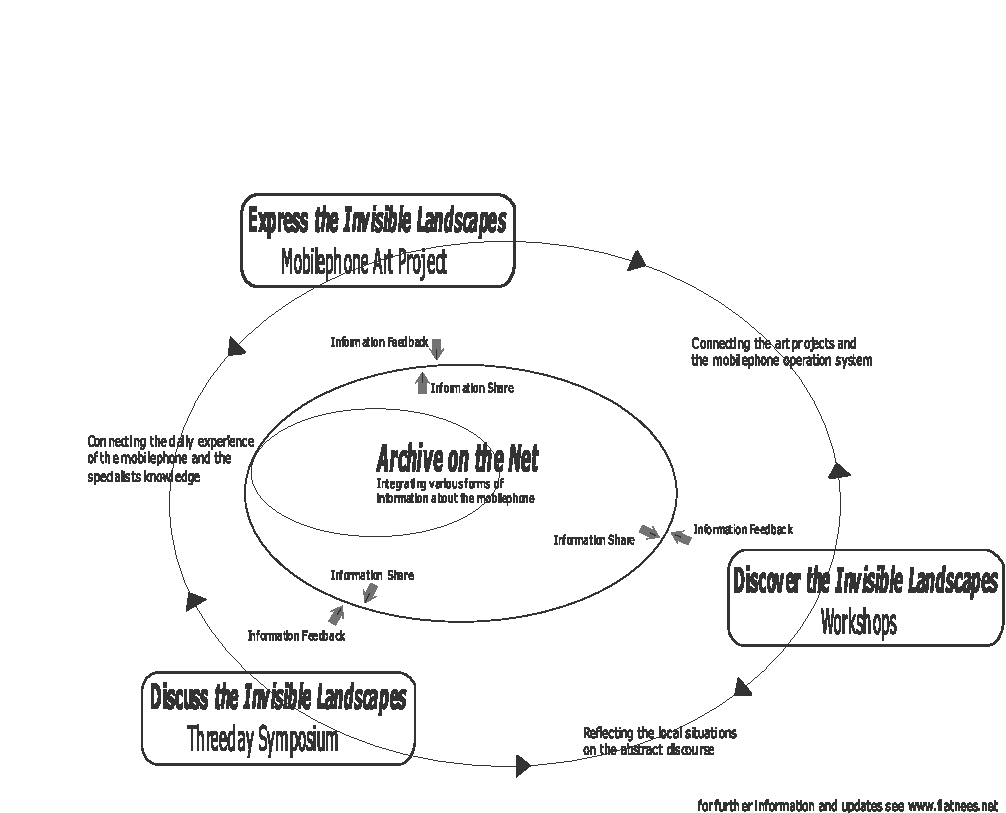
\includegraphics[width=\linewidth]{img/InvLandscape}
    \caption{Map of events for the project \emph{The Invisible Landscapes}.}
  \end{center}
\end{figure}
% \movetoevenpage

% This is a comment to the section collaborative music.

% \cleartorecto

\section{Collaborative music}
Collaborative musical compositions and sound art has been realized in
a number of ways and with different objectives. In the project
\emph{Norge - et lydrike, Norway Remixed} the curatorial idea was `to
bring the whole country together through sound', so `the local branch
offices of the broadcasting corporation' was supplying sound material
`in order to secure authenticity' and `actively counteract
speculations of centralisation' \footcite{rudi}. In their article on
\emph{The Interactive Dance Club} Ulyate and Bianciardi define the
goals as:(1) `to allow group and individual participation', (2)`create
a compelling social environment' and (3) to `deliver the euphoria of
the artistic experience to ``unskilled'' participants' \footcite{ulyate}.

These are just two examples in a very active art and music field.
Though their respective aims are different, they both share the
intention to create a soundscape that can communicate a sense of
solidarity. In the first case by introducing an awareness of the
political, and potentially exclusive aspects of music making already
in the curatorial concept. By letting a large number of individuals
supply the input, according to the article the work succeeds in
creating a fabric of references valid to a large number of visitors
and thus creating `building blocks of culture' \footcite{rudi}. In the
second case the visitors are offered to actively participate in the
familiar environment of a dance club. But instead of merely responding
in this environment the visitors are offered to influence the music
and imagery they are responding to, individually or collectively.
Action performed is not only the end result but also the initiation of
the next process.

Music making has traditionally been tied to the physical space,
whereas now, through the Internet there is a very active \index{virtual}virtual space
that has been explored for collaborative work in sound (\footcite[I.e.][]{barbosa, jorda99, duckworth}). To invite even amateur performers
to collaborative music making is a complex matter. But it is also an
agency to open up the creative process and opening up the creative
process for participation is a step towards interpretation and
perceptiveness, or as put by Jord\`{a}: `the best way to understand
and appreciate any discipline [\ldots] is by ``doing'' and being part
of' \footcite{jorda02}. The main intention with the collaborative element
in \emph{etherSound} was to let the desire to participate be the
driving force and the challenge therefore was to design an interface
that was as open as possible to anybody who had the wish to take part.

\section{The design of \emph{etherSound}}
The idea of making \emph{etherSound} a piece that required active
participation from the public grew out of the early discussions
surrounding the development of the general concept of the curatorial
project, \emph{The Invisible Landscapes}. \emph{etherSound} was first
imagined as a sounding body that derived its control from non-active
participation, specifically from data about activity in the GSM
network surrounding the exhibition space. Facing difficulties
regarding issues of information security, it became clear that mobile
phones could successfully be used in order to let the public interact
with the sound much more actively. \emph{etherSound} adopts the mobile
phone, maybe the most popular device amongst the new tools for
communication and opens a participation channel to the public.

The principle idea behind \emph{etherSound} became an attempt to
design an instrument that could be played by anybody who had the
knowledge to send an SMS (Short Message Service) from their mobile
phones. In the version displayed at \emph{The Invisible Landscapes},
all messages sent to a specified number were received by an Internet
server, parsed for its content, the phone number it was sent from and
the date and time it was received. This information was written into a
database which was queried at regular intervals by a computer running
a control and text analysis application (written in Java \footcite[See][]{j2se,
  j2ee}) and the sound synthesis \index{software}software (\index{Max/MSP}Max/MSP \footcite{max} running
a \useGlosentry{glos:csound}{Csound} orchestra \footcite{csound}). For every new message, the data was
downloaded, processed and analyzed by the control program, turned into
control signals which were then sent to the sound synthesis engine.
Every message generated one sonic object that would last for up to two
minutes. The response was very direct - a received SMS would result in
an immediate and perceivable change in the sound. \emph{etherSound}
was tried in two different modes: as a stand alone interactive sound
installation; and as a vehicle for improvisation. In the latter, one
or several performers improvised along with the sounds of the
installation while the audience contributed actively to the
performance by sending text messages.

% \begin{figure}
%   \begin{center}
%     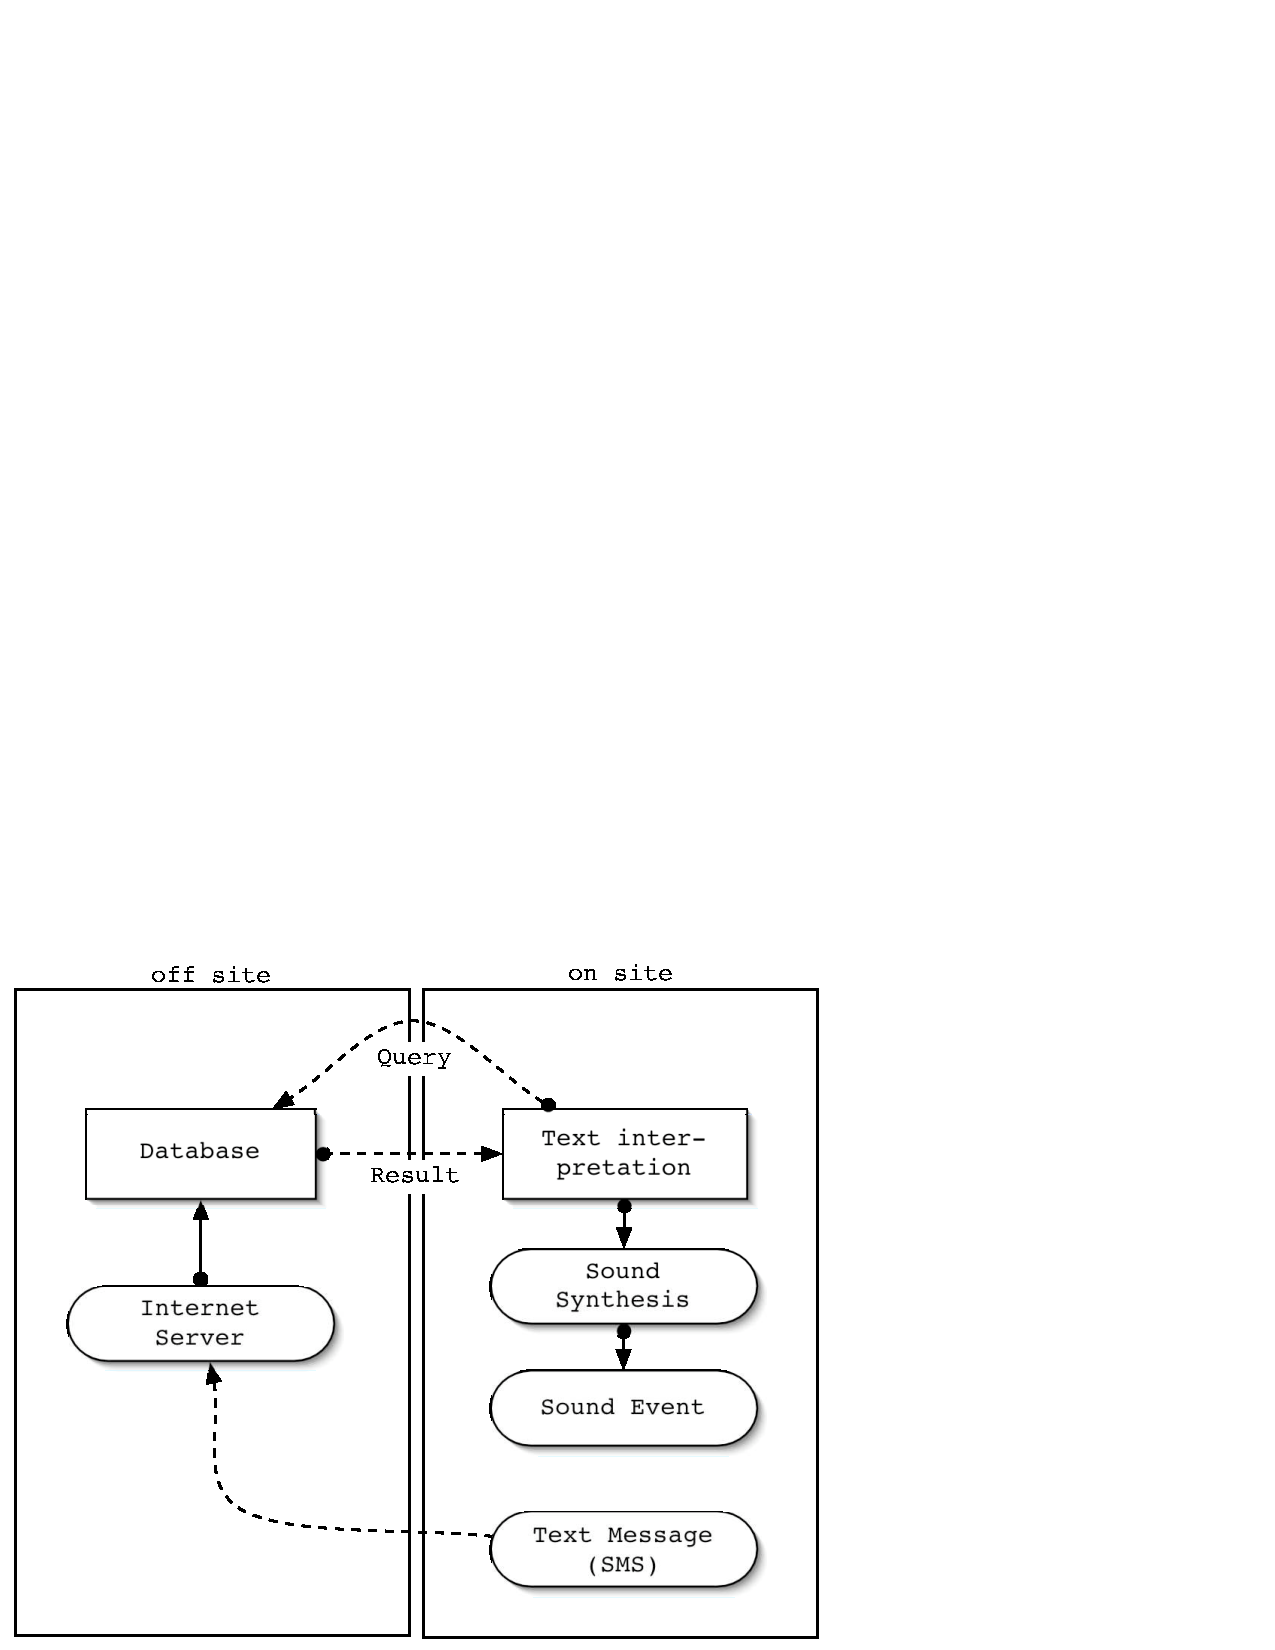
\includegraphics[width=0.7\textwidth]{img/FriskF2}
%     \caption{Diagram of the system for receiving and processing incoming SMS messages.} \label{comm}
%   \end{center}
% \end{figure}

In this work the mobile phone is the interface to the sound production
and to the distribution of sound events. The way the mobile phone is
used here, as a text only input interface, is rather limited and much
of the rest of this article evaluates the advantages the mobile phone
has, despite its limitations as a text input interface. If the only
purpose of etherSound was to allow users to input text that would be
transformed into sound, installing a computer with a keyboard that
would allow visitors to post messages on site would conceivably be
technically less complicated. Another solution, more dynamic than the
one we chose, would have been to implement a voice interface that
allowed for true real time interaction similar to that of the Auracle
project \footcite{auracle}. Although this last option was considered, such
a solution would need a technical and finacial framework that was
beyond our scope.

\section{Communication, time and creativity}
It has been suggested that young people's (specifically teenagers) use
of text messages (SMS), call-credit and mobile phones themselves can
be interpreted as a form of \emph{gifting}: `We will contend that
these gifts are exchanged in performances that have specific meaning
in young people's daily lives and are played out with the intent to
cement social relationships'\footcites[][]{taylor}[See also][]{marcel}.
In other words, text messages have a meaning to the sender and the
recipient that transcends the actual content or meaning of the
message. This is, in more than one way, in accordance with how the
messages sent to \emph{etherSound} were used. The content of the
message as such is not transparent in the resulting sound object, only
the general outline of it (the length, the composition, the number of
syllables, etc.) and every message is `rewarded' with sound; the gift
is always returned. To further develop the meaning of the returning of
the `gift' the temporal aspect of etherSound needs to be considered.

There are two time frames at play in etherSound which bear immediate
significance to this question and they are described here borrowing
terms from Curtis Roads table of temporal hierarchies in music
\footcite[3]{roads}: (1) The `meso time scale' which constitutes the
single message and the resulting sonic events. The mapping between the
message and the sound is linear and relatively consequent. (2) The
`macro time scale' which is the time from when the installation was
started to when it ends. It is within the meso time scale that the
relation between the object and the participant is established and it
is in the dynamics between the meso and the macro time scale that the
`returning of the gift' has curtial significance. It constitutes a
receipt of the contribution; a sonic confirmation that the message has
been received. This kind of immediate response is important in order
to avoid a sensation of exploitation in the participant: Their time,
energy and, in the case of sending text messages from mobile phones,
their money, is not used to fulfill our own opaque objectives hidden
to the participant, but results in a palpable response with a value of
its own. This is the main reason a clear causality between input and
output in the meso time scale is aimed for. Therefore, some effort has
been invested in making each sound object a closed form musical
composition in its own right. However, as soon as the sound object
begins to play back it transmutes into a player in the macro time
scale, in which there is no preconceived musical form but where the
indeterminacy of collective efforts are the main factor. It should be
noted that the relation between the closed form of the meso time scale
and the indeterminacy of the macro time scale is not unproblematic. An
interactive, ongoing and indeterminate, musical creation will
inevitably dismantle the traditional idea of musical form. There is
nothing new with the ``permanent event'' \footcite{barbosa} or the
infinite musical form but it is the effect the indeterminate form has
on the \emph{understanding} and \emph{interpretation}\footnote{Perhaps
  \emph{reading} would be a better word to avoid confusion with the
  musical term interpretation.} of the work from the point of the
participant, and whether the closed form of the message compositions
enhance or degenerate this effect, that is of interest. Will a random
collection of message compositions, each one with a sense of musical
form, generate a large scale (closed) form or will they result in
something else, conceptually different from musical form? I believe
both is possible and, in this particular case, they are both part of
the very core of the artistic intent. It is a question of
perspectives. By opening up the form, the listening experience is
likewise opened up and a multiplicity of perceptive perspectives
becomes possible. However, the most plausible interpretation regarding
the form of \emph{etherSound} is that it is indeed a closed musical
form, but in which the structure of the sounds is open and subject to
change. 


In the age of mass information, consumerist ideology and market
segmentation strategies, individuality is at stake. Laura Martz
asserts that `the \index{Spectacle, Society of the}\index{Debord, Guy!Spectacle}spectacle\footnote{Martz uses the term `the
  specatacle' with a reference to what Guy Debord and the
  situationists called `the society of the \index{Spectacle, Society of the}\index{Debord, Guy!Spectacle}spectacle'
  which includes commodities, art-as-commodity, the mass media and the
  entertainment industry. \cite[See also][]{debord56}} steals every experience and sell it back
to us, but only symbolically'\footcite{martz}, but we believe it is fair to
assume that the desire for personal and individual expression among
the general public and the wish to exercise influence has not
vanished. As we will discuss later, individuality taken too far can be
a problem in the context of an interactive collaborative work such as
the one discussed here, but it is also an asset. Along with curiousity
it is an incitement for wanting to participate, provided that the
action invested results in a perceivable stimuli.

The clear causal relation between the action invested and the sounding
result is a way of giving the participant an experience of involvment
that ultimately could lead to a wish to further explore the causality
of input and output, and give a sensation of understanding. The
suggestion by Taylor et al. that mobile phone originated text
messaging is already used in some circles for \index{interaction!social}social interaction
indicates that the mobile phone is indeed well suited as an interface
for interactive art work where the creativity of the participant is
the object.

\section{Technology, communication and understanding}
Concerning the ideology of the broadening of the audience, Mary J.
Jacob ponders that public participation in the public art of the 90's
never widened the audience \footcite{jacob}. Her contemplation hits a
point, but in order to evaluate the processes in play in our project
we need to consider the social dynamics of new communications
technology. As has already been stated, mobile communication is no
longer a luxuary reserved for the privileged classes, but accessible
to most citizens in the Western World. It may be proposed that luxuary
today is to \emph{not} be accesible, a luxuary that only the secure,
upper classes can afford.

About ten years ago, in the early ages of email communication it was
seen that the nature of the medium had effects on group dynamics:
\begin{squote}
  Advances in computing and telecommunications technology are changing
  how people can meet and make group decisions. Technological changes
  help people cross physical, social, and psychological boundaries and
  have secondary effects on group behavior and decision making.
  Experiments show that compared with face-to-face meeting, a
  computer-mediated discussion leads to; delays; more explicit and
  outspoken advocacy; "flaming"; more equal participation among group
  members; and more extreme, unconventional, or risky decisions.
  \footcite{kiesler92}
\end{squote}
Whether this is also true for SMS communication is a matter of
speculation but it suggests that the means of communication has far
stretching consequences that needs to be considered when designing
interactive interfaces for public art.

We believe that advanced technology, designed for the consumer market,
such as the cellular phone, leans itself well to the purpose of public
interaction and may also help to counteract the tendency for art to
turn itself to the already initiated. What Walter Benjamin
\footcite{benjamin} calls the `advent of mechanical reproduction of art'
has, according to DiMaggio et al., along with other things, `resulted
in a tendency for culture interests to diffuse across class lines'
\footcite{dimaggio}. Benjamin writes:
\begin{squote}
  Around 1900 technical reproduction had reached a standard that not
  only permitted it to reproduce all transmitted works of art and thus
  to cause the most profound change in their impact upon the public;
  it also had captured a place of its own among the artistic
  processes. \footcite[][chap. 1]{benjamin}
\end{squote}
What will be the impact upon the public of the new tools of
distribution of text, audio and images and what will be the role of
the present day technological devices used for communication within
the spheres of creativity and art production? It may not be possible
to answer these questions for many years, but we feel it is of great
interest to evaluate and experiment with the use of these tools within
the realm of artistic and creative expressions.

It may be presumed that consumer market technology, for economical
reasons, is designed to be accessible to as many people as possible
within the target segments assigned by the production companies. The
vast popularity of the mobile phone, despite its technological level
of complexity, coupled with the recent price drops of service charges
suggests that, for mobile phones, this is true. However it should also
be noted that certain segments of the western societies (notably
senior citizens) and the development countries, are still locked out
from, and largely ignored by, this communication revolution. This
taken into consideration, the dynamics of mobile phone usage and
accessibility nevertheless seems to be of a different class than that
of traditional culture consumption. If this holds true, constructing
an interactive interface to an art work based on the use of mobile
phones can potentially open the work to not already initiated groups
of the public.

\section{Creative production and space}
Even though \emph{etherSound} is not site specific in the traditional
sense, it may still be regarded as such since it follows the logic of
the flattened non-space of telecommunication. The phone is tied to a
\index{virtual}virtual space and \emph{etherSound} exists within this space as it is
delimited by the group of people interacting with the installation at
the very moment interaction takes place.  As a result, the context is
\emph{not} the gallery space, but the curatorial idea that delineates
\emph{The Invisible Landscapes}.

\begin{wrapfigure}{r}{0.6\linewidth}
\begin{center}
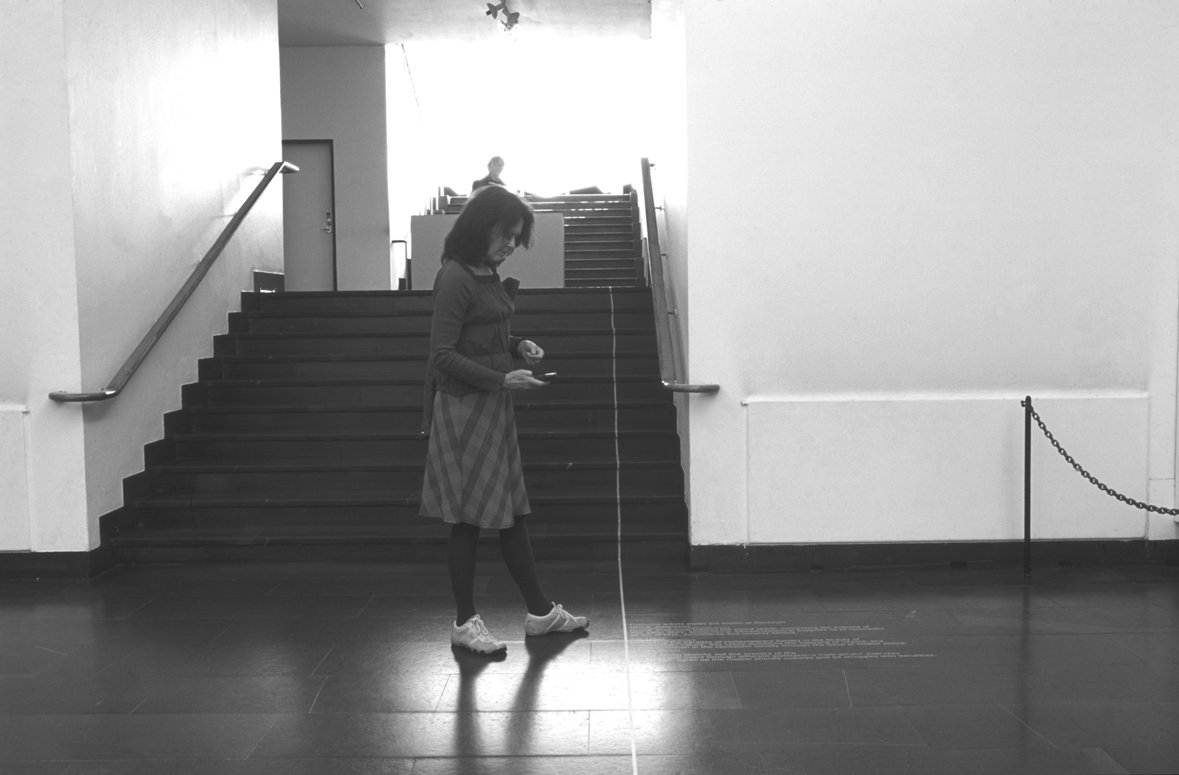
\includegraphics[width=\linewidth]{img/FriskF1jpg}
\caption{The space at Malm� Konstmuseum where \emph{etherSound} was first realized.}
\end{center}
\end{wrapfigure}
As we have discussed, the emergence of mobile communications, the
Internet and the technological devices that are used to interact on
these networks, has the potential to change the nature of (social)
participation. Now, participation takes place as an extension of
everyday acts. At its best, it does not matter if it is manifested and
glamorized as a single, unique and individual voice. It is not
strained and it is not in a pedagogic mode, but rather follows a mode
of pop culture. It abandons the rational individual and puts emphasis
on the collective in a typical Durkheimian fasion. We could say that
this new form of participation, consisting of clusters of anonymous
random acts, empowers a new structure for creative corporeality which
is never fixed within predetermined conditions but is more reminiscent
of a flow. We want to suggest that it holds potential as a new
coefficient of an autonomous agency of creativity.

The boundary between public and private in mobile phone communication
is not a straight line and can not easily be defined. If we take into
consideration the fact that it is possible to track the location of a
mobile phone, we may even go so far as to say that privacy ceases to
exist the moment ones mobile phone is turned on. But mobile
communication also makes possible a certain kind of private
interaction in the work domain as well as in public spaces. In their
article \footcite{taylor} list a number of circumstances where public
infringes upon private and vice versa. It may be suggested that the
space for mobile communication cannot be distinguished as private
\emph{or} public but creates a new space with its own set of
attributes. Taylor et al. writes:
\begin{squote}
  The phone and its contents, if you like, allows young people to
  differentiate themselves from family or household relations as well
  as cement their own social networks. The phone allows the young
  person to withdraw from the world of the home, for instance, and
  establish a ``micro-world'' through the system of exchange that
  young people employ. \footcite[292]{taylor}
\end{squote}

In \emph{etherSound}, a private act, the composing and sending of a
text message from one's own phone, is transformed to streaming sound
in public. Even though the content of the message remains hidden in
the public sphere, the processes it sets in motion takes place
publicly and may set in motion another private act. What was
originally private, and maybe even meant to stay private, affects the
public space and consequently, the participants share both the
physical and the imaginary, and the two feed off one another.

\section{Authenticity and interpretation}
Active public participation raises a series of questions about
authorship. Who is the composer and who is the performer? Who is the
originator? Who is the commissioner? In \emph{etherSound}, the creator
of the piece can very well be said to be the commissioner, and the
participants, supplying the input, the originators and the curator the
orchestrator. Or, the curator may be perceived as an originator, the
audience as the performers and the creator as the commissioner. We
believe it is impossible and of no use to impose pre-existing roles on
participants. Ultimately, the hybrid role created by different levels
of involvement should be in a state of flow in this work. The
coefficient of plural roles in one individual temporarily appears and
disappears in a subtle and sensitive balance, which, in every
performance will be different. It is `onceness' created by a new
coefficient through SMS participation.

Experience made from presenting \emph{etherSound} at a music
festival\footnote{\emph{Elektrisk Helg}, arranged by Ars Nova, held in
  Malm\"{o}, Sweden in April 2004} is testimony of the difficulty to
achieve this and of the importance of context. Musical performance is
surrounded by old and heavy traditions which implies a rigid
definition of the author. However, since the roles of the players
involved in \emph{etherSound} are interchangeable, confusion arose as
to what the music consisted of, which in turn resulted in some
performers doubting the validity of their participation.

Participating in \emph{etherSound} through SMS is an action started
from an individual initiation at the bottom level, that influences the
whole. The totality will further lead participation on to an
unpredictable outcome. It indicates the power of the situation and the
multitude (not an individual) as factors of creativity. Thus, the
attitude of conviviality naturally directs authenticity of the work in
a more flexible manner. There is no obvious author to credit, and this
opens up for a new form of authenticity, even in relation to
contemporary culture.

As has been noted, the content of a given message was not revealed in
the public sphere except as an abstract series of sonic events and
furthermore, and the audience was not informed of the mapping between
the message and the sound event it generates. This unkown relationship
between the SMS and the sound composition coupled with an expectation
of reflectivity stimulates the imagination of the participant and
navigates them towards a more careful attention to, and translation
of, the sound. This is consistent with Guy Garnett's analysis that:
\begin{squote} [\ldots] music can be roughly considered to be sounds
  made with aesthetic intent, or even sounds listened to with
  aesthetic interest. The former gives more weight to the role of the
  creator, while the latter formulation tends to privilege the
  listener\footcite{Garnett}.
\end{squote}
Hence, content is not only a result of a compositional process, but of
public active participation and in that sense there is nothing to
`understand' in \emph{etherSound} unless you participate. However, if
you do participate, understanding the resulting sound is not dependent
on a thorough insight of the history of art or electronic music
following the idea of the `telematic' piece:
\begin{squote} [\ldots] the observer in an interactive telematic system
  is by definition a participator. In telematic art, meaning is not
  something created by the artist, distributed through the network,
  and \emph{received} by the observer. Meaning is the product of
  interaction between the observer and the system, the content of
  which is in a state of flux, of endless change and transformation
  \footcite{Ascott}.
\end{squote}

\section{Conclusion}
Having discussed the positive effects that portable communication
devices can have in the context of public art it should be mentioned
that this mainly holds true in the Western World. Access to technology
and its uses can easily be taken for granted, but for certain groups,
even in the Western World, it is not self evident how a mobile phone
and all its options are operated, and tangled within this is the
danger of a new kind of class hierarchy based on knowledge of, use of
and access to communications technology.

In this project we have showed that the cellular phone, and its
owners' ability to send text messages from it, can successfully be
used as an interface for public interaction. We also believe that,
given our intentions, the SMS interface has some advantages compared
to other possible solutions. From a practical angle it is widespread,
comparatively simple to use, it is private and it is surrounded with a
large framework that makes it easy to integrate it in an artistic
work. In addition, in the Western World, it has already coalesced into
our private and professional lives and has become a tool for \index{interaction!social}social interaction. Participation can per se open up the work to groups of
people not familiar with contemporary sound art and an interactive
interface built around the mobile phone may contribute to in some
degree neutralizing the class hierarchies in arts consumption.

Even though interaction with \emph{etherSound} stems from an
individual wish to participate, the interface and the system center on
the public rather than the private. This transformation from private
to public opens up for a new sensation of space and an auspicious and
dynamic impression of creativity. Moreover we have suggested that
communication itself is a corresponding form of creativity.

A thought that was never implemented due to lack of funds and
technical equipment, was to, in addition to the location specific
installation, stream the sound on the Internet. This would allow for
groups of people that, for various reasons, did not have access to the
location of the exhibition hall, to participate and it would greatly
expand the accessibility. Further, it would be interesting to try to
allow for greater depth in the system and yield for `expert'
performance. This would however have to be done with great care in
order not to loose the collective focus.

%%% Local Variables: 
%%% mode: latex
%%% TeX-master: "../stim_create"
%%% End: 


% \chapter{Negotiating the Musical Work: An empirical study on the
% inter-relation between composition, interpretation and performance}
% \label{cha:negot-music-work}
% \epigraphhead[0]{
% \epigraph{This paper was first presented at the \emph{Electro-acoustic
%     Music Studies} conference in Beijing in 2006. The version printed
%   here is also published on the EMS Network
%   site.}{\citep{frisk-ost06-2}}}
% \begin{minipage}[t]{0.6\linewidth}
%   \begin{large}
%     \textbf{Authors:} \emph{Henrik Frisk \& Stefan �stersj�}
%   \end{large}
% \end{minipage}
% \section{Introduction}

In this article we outline the theoretical background for some of
the empirical studies performed within the frame of our respective
artistic PhD projects at the Malm� Academy of Music, Lund University.
The purpose of the studies performed and hence, the
requirements of the methods we use to perform them and study their
outcome, is to explore the inter-relations between performer and
composer. Specifically we study the musical work in
the Western art music tradition, prior to its ultimate
notation and prior to its performance. Though many of the
ideas presented below may apply to other genres this article is mainly
concerned with music for solo instrument and live electronics.

Trevor Wishart introduces the idea that the development of notation
has, among many other things, resulted in a division of the musician
into `composer' and `performer' \citep{wis96}. This split calls for an
extended discussion of what composer and performer provide to the
creative process. Our ambition is to approach this issue by studying
the low-level processes leading up to a version of the musical work.
We find that by using the concept of `agents' we bypass the otherwise
problematic values traditionally assigned to the two labours. The
musical work as an open concept, such as it is developed by Lydia
Goehr in her book \emph{The Imaginary Museum of Musical Works} (1992),
is also central to the reasoning in this paper as well as her claim,
that the work concept has had a regulative function only at certain
times in the history of Western art music. In contemporary music this
regulative function can be found to be pertinent in one composer's
work and extraneous in another's.

\section{The Ontology of the Musical Work}\label{sec:ontology}

A musical work, in the cultural context of the Western art music
tradition, and especially since the romantic era up to the present
day, is commonly regarded as the result of a process in two distinct
phases; one constructive and one reproductive. The composer produces a
score, which in turn is handed over to a performer who makes an
interpretation of the notation and reproduces it as specified in the
score. The score constitutes the primary source of information (see
Figure \ref{cons-rep}).

 \begin{figure}[!htb]
 \begin{center}
  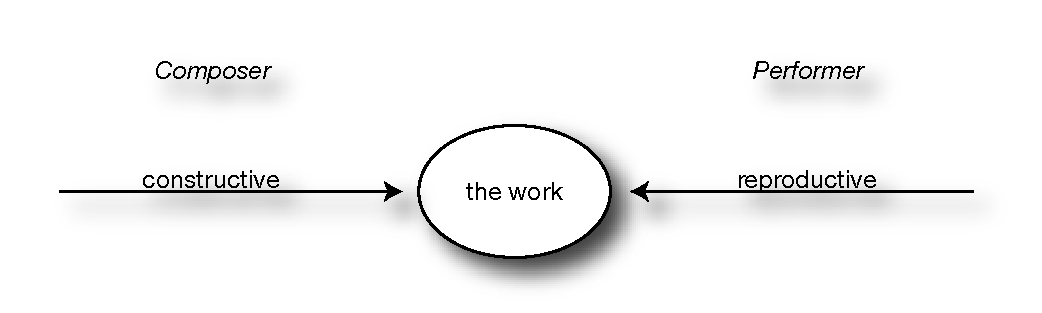
\includegraphics[width=0.8\columnwidth]{img/cons-rep2}
  \caption{Within the Western art music tradition the score is commonly
  regarded as the primary source of information.}
  \label{cons-rep}
 \end{center}
 \end{figure}

 In Paul Ric{\oe}ur's hermeneutic philosophy, the traditional view of
 the author as a one-way sender of a message is disputed. Ric{\oe}ur
 finds that the author is disengaged from the work by the act of
 writing \citep{ric91}. When writing takes the place of dialogue, the
 immediate face-to-face communication is replaced by inscription and
 the semantic autonomy of the text. The disconnection between the
 author's intention and the meaning of the text is a key issue in
 Ric{\oe}ur's theory. The inscription of a discourse in writing brings
 the semantic autonomy of language into play.

\begin{quote}
  The text is the very place where the author appears. But does the
  author appear otherwise than as first reader? The distancing of the
  text from its author is already a phenomenon of the first reading
  that, in one move, poses the whole series of problems that we are
  now going to confront concerning the relations between explanation
  and interpretation. These relations arise at the time of reading.
  \citep[p. 109-10]{ric91}
\end{quote}

Suppose that we undertake the hypothetical experiment of applying this
theory on the literary text to musical production: are there any
analogies between Ric{\oe}ur's account and musical practice? Imagine
music-making, as it takes place independently of musical notation, as
compared to the kind of dialogue that the inscription of text
replaces. Improvisation involves making variations on known patterns,
and when this is successful, truly innovative music comes out. Imagine
a composer writing music: Isn't it necessary for him to interact with
the musical `language', or context, in which he is working, in a
similar way as is necessary for the improviser? Analogically speaking,
the moment that the composer starts making the notation, the
'dialogue' is replaced by the semantic autonomy of the text-based
musical context, with its own structural possibilities and
limitations. The composer is detached from the music in the act of
notating it. In the case of a written text, the intention of the
author is not equal to the meaning of the text. The author is present
in the text, but only as a first reader. Similarly, this suggests that
the construction of a score-based work consists of dialectic interplay
between creation and interpretation, in which the composer - even
during the act of writing - has to approach the notation by means of
interpretation.

By this reflection on the artistic process, and in the light of
Ric{\oe}ur's philosophy, the view of the composer representing the
productive phase, and the performer the reproductive, is questioned.
We arrive at a modification of the traditional scheme of
construction/reproduction, instead involving construction, but also
interpretation in the composer's creative process.

\begin{figure}[!htb]
  \begin{center}
    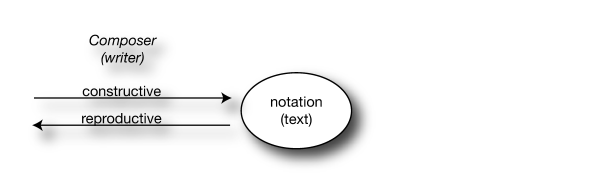
\includegraphics[width=0.8\columnwidth]{img/cons-rep-ric2}
    \caption{In the light of Ric{\oe}ur we arrive at a modified scheme
      involving construction as well as interpretation in the composer's creative
      process.}
    \label{cons-rep2}
  \end{center}
\end{figure}

Another aspect of the composer's practice is highlighted by
Horacio Vaggione \citep{vaggione01}. The composer always has to
approach the process of producing a piece of music as a listener,
either in the form of inner listening while writing an instrumental
score or the concrete listening in the production of a pure electronic
piece. This is described by Vaggione as an action/perception feedback
loop, reminiscent of the notation/interpretation process suggested by
the thinking of Ric{\oe}ur. But there is a fundamental difference
between the two accounts: what Vaggione provides is a theoretical
reflection on the kind of thinking that is not based on language, but on
action and perception.

\begin{quote}
 In order to produce music an act of hearing is necessary, whether it
 be the `inner hearing' (the silent writing situation) of pure
 instrumental music composition, or the `concrete hearing' of
 electroacoustic music composition. These situations involve variants
 (there are many others) of an `action/perception feedback loop' which
 can be defined as an instance of validation proper to musical
 processes. \citep{vaggione01}
\end{quote}
Without any further specification, Vaggione hints at the many other
 variants of this class of feedback loops at play in the production of
 musical content. It is important to bear in mind that `thinking' in
 modes of action does not require a `transcription' into language.
 What Vaggione reminds us is that `thinking through hearing' and
 `thinking through performing' are essential modes of interpretation.
 These involve the physical interaction between a performer and his or
 her instrument as well as the inner listening of the composer; both
 of which do not require verbal translation. This kind of
 interpretation is what we would call `thinking through
 practice'.\footnote{One important source for the notion of `thinking
   through practice' is the thinking of Art historian and curator
   Sarat Maharaj. His introductory paper for the \emph{Knowledge Lab}
   at the \emph{Haus der Kulturen der Welt in Berlin} 2005 (in which both
   authors participated) was entitled `Thinking Through Performance'
   and discussed how various modes of `thinking through' could
   function as a methodology for the creation of new knowledge in the
   arts. We believe that the way we use the term in the present paper
   makes a slightly different use of the notion of `thinking through':
   in the \emph{Knowledge Lab}, `thinking through' referred to a mode of
   studying artistic practice, whereas we use the notion to describe
   processes within artistic practice itself. One could argue that
   our study gives further confirmation to the methodology suggested
   by Maharaj for the \emph{Knowledge Lab}.}

Our conclusion is that the
 use of notation and the subsequent musical practice that has followed
 from it, does not unambiguously divide composer and performer into
 one `auteur' (producing the work) and one interpreter (reproducing
 it). Interpretation is a part of both creative acts and the
 practices of both agents overlap in many ways.

\begin{figure}[!htb]
  \begin{center}
    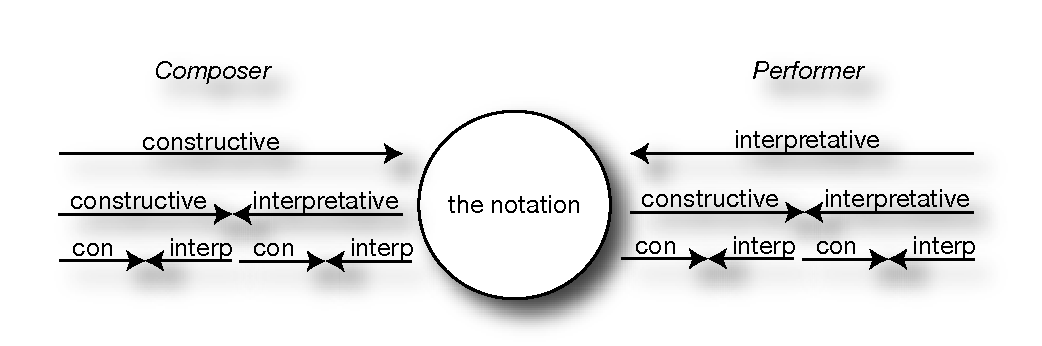
\includegraphics[width=0.8\columnwidth]{img/cons-rep-rep-cons2}
    \caption{Our schematic model of the interaction between
      constructive and interpretative phases in performance and
      composition.}
    \label{cons-rep3}
  \end{center}
\end{figure}

\subsection{Musical Interpretation and performance} \label{subsec:musical_interpretation}

Since the 19th century, performances of score-based works have
commonly been referred to as interpretations. If we regard
performances as interpretations, are they interpretations of the
notation or of a wider entity? This is in essence a matter of the
ontology of the musical work: Is the work equivalent to the score or
is there more to the identity of the work than notation? According to
Theodor Adorno, the ``musical score is never identical with the work;
devotion to the text means the constant effort to grasp that which it
hides [...]'' \citep[p. 144]{adorno81}. A crucial fact about musical works
is their historicity. Firstly in the sense that the material that is
available to the composer is historically and culturally mediated and
thus pre-formed within the cultural context in which he is working.
Secondly, meaning in music, and in Adorno's view this also equals the
musical work itself, is achieved in the tension between the received
formal norms and the `second reflection' or re-contextualisation in
the compositional process by the creative `Subject' \citep{pad91}. The
work is not equivalent to the score but is a cultural construct that
materialises in its relation to its cultural context.

Paul Ric{\oe}ur introduces the concept of the `world of the text' as
something other than the intention of the author. The meaning of the
text is projected in front of the text, and is not to be found in
authorial intent `behind' the text, as in romantic hermeneutic
philosophy. What is unfolded by the passing from explanation to
understanding is the thing of the text, or the kind of world that the
text unfolds before the text.

\begin{quotation}
Reading is no longer simply listening. It is governed by codes
comparable to the grammatical code that guides the understanding of
sentences. In the case of the narrative, these codes are precisely the
ones that a structural analysis brings to light under the title of
narrative codes.

It cannot, therefore, be said that the passage by way of explanation
destroys intersubjective understanding. This mediation is required by
discourse itself. I am expressly using the term discourse and not
simply speech, the fugitive manifestation of language. For it is
discourse that calls for this ever more complicated process of
exteriorization with regard to itself, a process that begins with the
gap between saying and the said, continues through the inscription in
letters, and is completed in the complex codifications of works of
discourse, the narrative among others. Exteriorization in material
marks and inscription in the codes of discourse make not only possible
but necessary the mediation of understanding by explanation, of which
structural analysis constitutes the most remarkable
realization. \citep[p. 130]{ric91}
\end{quotation}

Not only is the author detached from the work by the act of writing.
For a reader to enter into the world of the text, a similar process of
detachment and analytical interpretation is needed. But writing music
is an activity distinct from writing a literary text. A score, to a
higher degree than is a text, is a tacit agreement with a present or
implied performer - we cannot simply equal a verbal text to a score and
a performer to a reader of this text. But there seems to be an
immanent call for analysis and interpretation in the construction of
musical meaning. Musical meaning may be found through a movement from
explanation through analysis to understanding.

\begin{quotation}
The performance of a piece of music is (...) the actualisation of an
analytic act - even though such analysis may have been intuitive and
unsystematic. For what a performer does is to make the relationships
and patterns potential in the composer's score clear to the mind and
ear of the experienced listener. \citep[p. 29]{meyer73}
\end{quotation}

From a general point of view, interpretation in the context of the
arts can be understood as assigning meaning to works. To what
extent can we claim that performances do this? Turning to definitions,
we will now attempt to trace the difference between critical
interpretation and what we tend to call performance interpretation.
\begin{quotation}
Being an interpretation of is a relation between a thought or an
utterance on the one hand and an object of interpretation on the
other. In the case of art (...) an utterance about a work is an
interpretation of the work, only if it says something about the
meaning of a work, about a meaning it could have or was intended to
have, or about the work's significance. \citep[p. 82]{stecker}
\end{quotation}
Stecker's definition of interpretation raises some important
questions: What musical actions do we regard as interpretation, and in
what sense do they assign meaning to the work? 

Are the performer's shaping of phrases, relative level of dynamics and
accents etc. really to be regarded as an interpretation of the piece,
assigning meaning to the music? Markings by the composer of dynamics,
accentuation, phrasing etc are often regarded as `interpretative'.
This mode of speaking implies that markings of this kind represent the
author's interpretation of the meaning of the work. But this seems
implausible to us. Isn't it more likely that the reason we tend to
regard these markings as interpretational is that they represent a
category of musical organisation that often has been left to the
performer's discretion? According to our understanding of the musical
event all parameters belong to the musical fact.

In the preparatory stages the performer has to make decisions of a
kind that do not clearly differ from that of critical interpretation
\citep[38-9]{levinson}. In order to take a position in cases where a
score is incomplete, inconsistent or exists in different versions, a
critical interpretation of the score is necessary. This could imply
that the difference between critical and performative interpretations
is of a floating and unclear kind. On the contrary Levinson argues
that they are logically distinct activities.

\begin{quotation}
...a critical interpretation typically aims to explain (or elucidate)
a work's meaning or structure - "what is going on in it", in a common
phrase - whereas a performative interpretation can at most highlight
(or effectively display) that meaning or structure. A performative
interpretation, if successful, may enable one to conceive of a work
differently in the critical sense - as the performer conceived it in
arriving at the performative interpretation - but only a critical
interpretation indicates or details such a conception. \citep[p. 38-9]{levinson}
\end{quotation}
In other words, there are many ways in which a performance fails to
fulfil the criteria for a critical interpretation. In critical
interpretation we do not have this peculiar amalgamation of `object of
interpretation' and the `interpretation' itself. This crucial
difference between performance and critical interpretation is also
acknowledged by Robert Stecker:
\begin{quotation}
If performances and critical interpretations are both representations
of works, they are so in quite different senses. If we ignore these
differences, we can easily be misled to make invalid inferences.
Performances are necessarily constructive; that is, they necessarily
add features that the work leaves vague or undetermined. \citep[p. 80]{stecker}
\end{quotation}
But not only in cases in which the notation is in some respect unclear
or vague is there a call for constructive elements in performance.
Construction is really at the heart of the matter. The relation
between a performance interpretation and the work is not the relation
between an external receiver and an artwork but the relation between
different forces at play in the construction of the work itself. The
use of notation presumes a common understanding of performance
practice of composer and interpreter. This fundamental agreement
between a composer and an imagined or present performer is part and
parcel of every musical notation. As we have seen in the thinking of
Adorno and furthered into the model of `the world of the text', a true
instance of a work must be based on an interpretation that goes beyond
the mere text of the score. Assigning meaning to a musical work is
achieved by way of a critical reading of the work (and not only the
score). Musical meaning is constructed in the relation between the
musical structures themselves and the musico-historical context - its
tradition - and the friction between this context and the work.

In the preservatory culture that Classical Music is today, we tend to
speak of works as ideal objects that are `interpreted' in performances
that can be evaluated in comparison with this ideal entity. However,
we find that musical interpretation is better understood as an
analytical and hermeneutic tool that is a part of the agencies of the
performer as well as the composer. Performances are not separate from
the work but always a part of it - a successful performance is an
embodiment of the work\footnote{This is not to say that performances
  cannot be more or less true to the instructions in the score, or to the
  tradition, and that the performance itself should not be accessible
  for critical consideration.}:
\begin{quotation}
Every performance is an event, but not one that would in any way be
separate from the work - the work itself is what `takes place' in the
performative event.\citep{gad60}
\end{quotation}
We would like to propose the fairly radical idea of dropping the term
performance interpretation. Preceding performance is an act of
interpretation, either by means of analytical thinking (critical
interpretation) or through an embodied mode of `thinking through
practice'. However, it is important to bear in mind that, just as
Gadamer reminds us, a performance is not to be understood as an
interpretation of a work, but as its final constructive phase.

\section{Musical semiology}\label{sec:musical_semiology}

In his 1989 article `Reflections on the development of semiology of
music' Jean-Jacques Nattiez offers an excellent review of the history
of musical semiology. In it he gives an historic perspective on the
fundamental issue of the nature of musical signification. Nattiez
distinguishes between intrinsic and extrinsic significations within
musical semantics, finding the theory of the former to be to a large
extent founded on the work of Nicolas Ruwet and the notion of music as
a language that signifies itself \citep[p. 30]{nat89}. Jean Molino
summarizes Susanne Langer's idea of music as the `unconsummated
symbol' and captures the essence of the problem: ``On the one hand,
the unchallengeable presence of evocation; on the other, the
impossibility of exploiting it'' \citep[p. 126-7]{molino}. Molino aims
at a theory in which music is understood as networked communication or
exchanges between individuals. As we will discuss more thoroughly in
the next section, the sender and receiver do not have to come to the
same understanding of the message, or the `trace' as Molino would call
it, hence there is no need for a understanding of the `code' which is
significant to the semiosis favored by Umberto Eco. Eco points to the
problems with connecting the investigation of a sign with the object
to which it refers. It is impossible to attribute logical statements
such as `true' or `false' to the semiological investigation of music
and for Eco these are pre- or postsemiotic problems; ``The signs are
of interest to semiotics as social powers'' and further ``Any attempt
to establish the referent of a sign will force us to define this
referent with the terminology of an abstract entity.'' This is what
Eco calls the ``cultural convention''. \citep[p. 61-6]{eco71}

Defining a cultural context as the referent resolves some issues in
the analysis of performed music as a social fact. The listener or
concert-goer can be defined as belonging to a cultural entity with
predetermined understandings of the context of the performance, but
also of the cultural markers within the music. This cultural entity
may then be used as a code to decipher the message (the music as a
symbolic system). However, in our study we are looking at a not yet
existing work - a work in progress - and we are not primarily
interested in the symbolic understanding of \emph{music} as it is
materialized in the physical world. Our focus is geared towards the
understanding of the \emph{actions} that lead to production of musical
content. Following Eco's model we might try to approach this symbolic
system in relation to a common context, or subculture created by the
agents involved in it. Both composer and performer are working within
the frame of their own cultural contexts which defines their
respective understandings of the evolving work. The subculture is a
result of interaction, and negotiation ('\emph{What is it we are
 developing?}', '\emph{How are we talking about it?}', etc.), between
the two agents and their inherent cultural contexts. Their mutual
expectations and their understanding or imagination of the work in
progress is of importance when they attempt at co-ordinating their
actions, for instance towards a definition of the performance
instructions. The musical work becomes the sign or the message, the
agents the signifiers and the subculture the signified. Where,
traditionally, we may tend to regard the composer/performer relation
as a hierarchic structure in which the role, even the purpose, of the
performer is to fulfill the composer's intentions (whether he is dead
or alive), this mode of analysis allows us to look at the two agents
as part of a larger system that may also contain many other agents.

But to fully understand the dynamics of the context, or subculture as
we call it, we also need the tools to move to a lower level of
analysis. The tripartite model suggested by Molino for analysis of
music, though certain aspects of it remains problematic, appears to be
a flexible method for our study at this stage.

\subsection{The three dimensions} \label{subsec:threedim} Molino
reminds us that the hypothesis that there is a ``single, well-defined
item of information to be transmitted, all the rest being simply
noise'' is ``dangerously inaccurate and misleading as soon as we move
from the artificial communication of information to a concrete act of
human communication as a total social fact.'' \citep{molino} Music,
according to him, is a product and not a transmission. The Duchampian
notion of a work of art is very similar; as two poles with the artist
on the one side and the viewer on the other - the intention of the
artist holds no significance to the work's interpretation. Molino
further refers to Paul Val\'{e}ry, to point out that ``there is no
guarantee of a direct correspondence between the effect produced by a
work of art and the intentions of its creator''. The distinction
between what was later coined as the `poietic' and 'esthesic'
dimensions in the symbolic phenomenon was first suggested by
Val\'{e}ry in his inaugural lecture for the Coll\'{e}ge de France in
1945.

The ambition of musical semiology has been to provide tools for an
analytic understanding of the total symbolic fact of the musical work
\citep[p. 34]{nattiez}. Molino argues for a three level symbolic
analysis; ``the poietic, the esthesic and the `neutral' analysis of
the object'' \citep{molino}. Three modes of analysis all representing
the same work of art. The analysis at the different levels does not
necessarily have to lead to the same conclusions or results but,
according to Nattiez, it may help us to understand \emph{all} aspects
of the musical work:

\begin{quotation}
...recognizing, elaborating, and articulating the three relatively
autonomous levels (poietic, neutral and esthesic) facilitates knowledge
of all processes unleashed by the musical work, from the moment of the
work's conception, passing through its `writing down', to its
performance. \citep[p. 92]{nattiez}
\end{quotation}

Leaving the problematic concept of the neutral level aside\footnote{It
  has been extensively debated elsewhere, see footnote 8 of \citep[p.
  35]{nat89} for a list of references}, a rudimentary definition of
the two terms `poietic' and `esthesic' from a musicological point of
view indicates that an analysis of the (external) poietics of the work
takes ``a poietic document - letters, plans, sketches'' as its point
of departure whereas an analysis of the (inductive) esthesic ``grounds
itself in perceptive introspection'' - that which is ``perceptively
relevant'', that which one hears \citep[p. 140-3]{nattiez}. The three
``families of analysis'' correspond to a:
\begin{quotation}
semiological `program' [...] that has three \emph{objects}:
\begin{enumerate}
\item the poietic process
\item the esthesic process
\item the material reality of the work (its live production, its
  score, its printed text, etc.) - that is, the physical traces that
  result from the poietic process.
\end{enumerate}
\citep[p. 15]{nattiez}
\end{quotation}
Though the `material reality' and the `physical traces' are not as
self evidently defined as a result of only the poietics of the work,
it is the processes themselves rather than the analysis of the
processes that are of interest to us in this paper. (In the study that
we performed following the methods developed here it will also be
clear that neither the poietics nor the esthesics belong to only one
aspect of the work.) The term `poietic' can be traced to the Thomistic
philosopher \'{E}tienne Gilson whose definitions are less concerned
with the analysis and more with the actual processes. According to
Nattiez:
\begin{quotation}
With `poietic' Gilson understood the determination of the conditions
that make possible, and that underpin the creation of an artist's work
- thanks to which something now exists which would not have existed,
except for them. \citep[p. 12-3]{nattiez}
\end{quotation}
Taking this short statement as a definition it may be argued that also
acts of interpretation (and analysis) involves a poietic dimension.

Nattiez further discusses the issue of where the poietic process ends
and the esthesic begins in score-based music (\emph{ibid}, p. 72).
For Nattiez this is in essence an ontological discussion: What is the
musical work, is it the graphic sign alone or is the musical work
incomplete before it is realised as sound in performance? Contrary to
our discussion in Section \ref{subsec:musical_interpretation}, Nattiez
finds that the greatest difference, between the score and the acoustic
trace left by a performance, is that while the score is ``an
invariable physical reality'' there are just as many acoustic
realisations as there are performances. The performance is the
borderline between the esthesic and the poietic field. By focusing on
the act of interpretation as it is performed between the score and its
sonifications (``the interpretants that insinuate themselves between
the score and its performance'' (\emph{ibid})), he draws the
conclusion that analysis of the neutral level has to be applied to
``the graphic sign alone, because that sign \emph{precedes}
interpretation'' (\emph{ibid}). Where Nattiez sees the production of a
musical work as a linear process, we tend to regard it as an
oscillating interaction between \emph{all} of the different agents
that are involved in the process, though, in this article, we limit
the discussion to include only the performer and the composer.

As we suggested in section \ref{sec:ontology}, the process of writing
down a musical work \emph{is not} a unidirectional poietic process but
should rather be understood as an interaction between esthesic and
poietic processes. This to an extent that makes it difficult to define
the end of the poietic process as well as the beginning of the
esthesic. The acts of musical composition that Nattiez gathers within
the poietics can in themselves be analyzed by using the same method
that he applies to the total fact of the musical work. According to
us, Nattiez gives too little consideration to the generative processes
(to repeat the quote: ``from the moment of the work's conception,
passing through its `writing down', to its performance'' \citep[p.
92]{nattiez}), articulating the problem in ontological terms. It
seems that Nattiez draws conclusions about ``processes unleashed
by the musical work'' from a purely analytical understanding of music.
This perspective is still dependent on the view of composers as `true
creators' and works as `ideal objects': stable and fixed artworks that
should make up the primary object of study for musicology.

What we are concerned with in these studies is almost the opposite: To
understand the actions that \emph{lead to} musical content and the
significance of the interactions between the agents involved in these
processes. A description of the generative phase of musical production
preceding notation might provide a better understanding of the nature
of the musical work evading the detour into abstract ontological
reasoning. Hereby we also avoid the difficult and much debated
issue of music as a signifying system.

\section{Discussion}

\begin{quotation}
  \begin{textit}
    {Just as the reading of the modern text consists not in receiving, in
      knowing or in feeling that text, but in writing it anew, in crossing
      its writing with a fresh inscription, so too reading this Beethoven is
      \emph{to operate} his music, to draw it (it is willing to be drawn)
      into an unknown \emph{praxis}.}
  \end{textit}
  \citep{barthesMus}
\end{quotation}
\nocite{barthes1}

What we are pointing at in this text is the possibility that not only
interpretation (in the sense that Barthes talks about it) is about
\emph{operating} the (musical) text. Also composition and the
processes unleashed by the `thinking through hearing', is about
operating the inner text of the imagination of the music. Furthermore,
we argue that this is an activity that, not only in collaborative projects, is
performed in negotiations between multiple agents.

In a study performed by the authors using the theory and method
developed in this paper the following conclusions were
drawn\footnote{For an in depth description of the empirical studies
  performed see \citep{frisk-ost06}.}:
\begin{enumerate}
\item Composition may be regarded as a complex interaction between
      esthesic and poietic processes.
\item Performers may similarly be said to oscillate between these two
      modes of artistic activity.
\end{enumerate}
By examining one particular event in one of the empirical studies
mentioned above we will now try to elaborate on these conclusions and
attempt to contextualize the reasoning in section
\ref{subsec:threedim}. The event is taken from a video documented
session with Swedish composer Love Mangs and guitarist Stefan
\"{O}stersj\"{o} in which they are working on \emph{Viken},
a composition for guitar and electronics. The session took place less
than two months before the premiere of the piece. S.{\"O}. has
improvised and notated a short musical fragment and L.M. is trying to
make S.{\"O}. to shape the melody differently by introducing the
notion of a fermata. At this point the roles are seemingly swapped;
the performer is notating music and the composer is thinking about the
interpretation of this musical fragment.

On his esthesic perception of the melody as it is defined by S.{\"O}.,
L.M. presumably wishes for a certain passage to be extended in time.
At first his suggestion about the fermata is not clearly understood by
S.{\"O}. The situation and the following communication indicates that
L.M. isn't really interested in a fermata in the classical sense - he
is merely interested in a different rhythmic contour of the melody.
(This confusion is likely to be one of the reasons his message is not
being comprehended by S.{\"O}.)

What follows is a negotiation between the two agents to establish the
meaning of the message `a fermata'. In this process they are both
active in the esthesic domain. However, if we move to a lower level of
analysis the suggested fermata can be seen as a poietic process
introduced by L.M., the meaning of which is being determined by
S.{\"O}. in an esthesic process. The importance here is not, not in
this paper nor in the session analyzed, to establish the denotation of
the musical term \emph{fermata}. Different musical performance
traditions will always hold different signifiers to the idea of the
fermata. But to fully understand the signifier of the idea of the
fermata in the context of \emph{Viken} as the idea is put forward by
Love Mangs, we need to understand what is signified by it
independently of the poietic (and esthesic) processes that led to its
inclusion, as well as in relation to the (sub)cultural context of the
collaboration between S.{\"O}. and L.M. This is what Eco would call
the `cultural history' and the `philological aspect' respectively both
pointing at the code used to encode the message \citep[p.
154-5]{eco71}. In this short example it is interesting to note that
the receiver as well as the sender is active in working out the code
used to encode as well as decode the message ('a fermata'). This
'working out' of the code is the process that in effect leads to the
abstract definition of the cultural entity, the \emph{subculture},
that becomes the referent of the musical work in question. At the end
of this process of negotiation a mutual understanding of the function
of the fermata in this specific context is established (which actually
goes well beyond the specific meaning of the symbol `fermata').

This session is also a useful example of how interpretative processes
of several kinds overlap and interact. When using improvisation to
develop new material it is evident that a greater part of the
hermeneutic processes are performed by various modes of `thinking
through practice'. However, as soon as notation is introduced,
also analytical modes of thinking make their way into the
continuous performing and listening of the two agents.

We suggest that musical interpretation can be divided into two kinds,
one based on language and analytical modes of thinking, the other
based on thinking-through-practice. According to Ric{\oe}ur, the act
of writing detaches the writer from the meaning of the text and our
claim is that this also applies to the act of writing a musical score.
Vaggione's notion of action/perception feedback loops captures a
characteristic feature of the composer's practice. This kind of
'thinking-through-practice' on the part of the composer may be
described as made up of mutually interactive poietic and esthesic
processes. We suggest this may be regarded as a hermeneutic process
making up a parallel species of interpretation at play in the
production of musical content. These various interpretative modes is
what we refer to as `thinking-through-practice'. Finally, the combined
efforts of all the agents involved in the construction of the musical
work creates the (sub)cultural entity that signifies that work.

From the above discussion of the ontology of the musical work and the
function of musical interpretation in the production of musical
content we make the following claims:
\begin{enumerate}
\item Musical interpretation can be divided into two kinds: `thinking-through-practice'
and analytic (critical) interpretation.
\item Interpretation plays a crucial role in the practice of both the
composer and performer.
\end{enumerate}

In this paper we have presented a method for performing studies on
the low level processes in the production of musical content. We have
showed how the perhaps somewhat dated and endlessly debated
semiological terminology by Molino and Nattiez may still prove to be
helpful at bridging the gap between disparate activities in the
field of musical production. The complex web of actions by several
agents in the production of musical content demands that the methods
used be flexible and responsive to the multiple layers of musical
practice. Though our proposed method needs to be thoroughly evaluated
and tested in practice it is our hope that these first steps taken
will prove useful for further development.

%%% Local Variables: 
%%% mode: latex
%%% TeX-master: t
%%% End: 


% \chapter{\emph{libIntegra}: a system for software-independent multimedia module description and storage}
% \label{cha:libint-syst-softw}
% \epigraphhead[0]{
% \epigraph{This paper was presented at the \emph{International Computer Music
%   Conference} in Copenhagen in 2007 and appeared in print in the
%   conference preceedings.}{\citep{frisk-bull07}}}
% \begin{minipage}[t]{0.6\linewidth}
%   \begin{large}
%     \textbf{Authors:} \emph{ Jamie Bullock \& Henrik Frisk}
%   \end{large}
% \end{minipage}
% \begin{abstract}
  In this paper we describe a means of storing information about audio
  and message processing modules, which is not software specific. This
  information includes a module description, module instance data, and
  module implementation data. A novel XML file format and database
  schema are proposed, and we show how a newly developed library
  (libIntegra) can be used as a link between persistent storage on a
  networked server, and an existing software environment for audio.
  The library provides methods for instantiating and connecting
  modules in a given piece of software, and addressing them using Open
  Sound Control (OSC) messaging.
\end{abstract}

%%% Local Variables: 
%%% mode: latex
%%% TeX-master: "../IntegraICMC"
%%% End: 

% % \newcommand\T{\rule{0pt}{2.6ex}}
% \newcommand\TT{\rule{0pt}{3.6ex}}
% \newcommand\B{\rule[-1.2ex]{0pt}{0pt}}
% \newcommand\BB{\rule[-2.2ex]{0pt}{0pt}}

\section{The Integra project}\label{sec:introduction}

libIntegra is part of the Integra project, a 3-year project led by UCE Birmingham Conservatoire in the UK and part financed by Culture 2000.\footnote{\url{http://www.integralive.org}} The Integra library is being developed as a foundation for the software development aspect of the project. 

\section{Integra modules}\label{sec:modules}

The basis of the Integra library is the concept of the Integra module. Integra modules encapsulate a specific piece of message or signal processing functionality. A module could perform a simple task like a numeric addition, or a complex task like emulating a specific synthesiser. In this section, we will outline how Integra modules and module collections are constructed.

\subsection{Module construction}\label{subsec:module_construction}

The minimum requirement for an Integra module is that it must have an interface definition. In addition, it may also have an implementation and module instance data. Of these, only the implementation is software specific.

\subsubsection{Module definition}\label{subsubsec:module_definition}

An Integra module definition is data that defines what attributes a
module has, and what the characteristics of those attributes are. An
Integra attribute is a symbolic name with which a value can be
associated. The module definition does not store the actual values of
attributes, instead it stores data about the attributes such as their
names, descriptions, supported data types, maxima and minima, and
default values. Typical module definition data is shown in Table
\ref{tab:module_definition}.

\begin{table}
\begin{center}
\begin{tabular}{|l|l|}
\hline
\textbf{Field} & \textbf{Value} \\
\hline
Name  & Oscillator \\
\hline
Parent  & Module \\
\hline
Attributes & freq, phase \\
\hline
Attribute Unit Codes & 1, 2 \\
\hline
Attribute Minima & 0, 0 \\
\hline
Attribute Maxima & inf, 6.2831853071795862 \\
\hline
Attribute Defaults & 440, 0 \\
\hline
\end{tabular} 
\end{center}
\caption{Integra Oscillator interface definition}
\label{tab:module_definition}
\end{table}

The parent field is used to show an inheritance relation. All Integra module definitions could be thought of as class definitions, the members of which are all abstract (lack implementation), or interface definitions. The interface of a given class can inherit the interface of any other class, and supplement this with additional members. This definition hierarchy is the basis of the Integra database (see section \ref{subsec:serialization}). 

\subsubsection{Module namespace}\label{subsubsec:module_namespace}

A module's namespace is derived from its definition. The namespace
enables the values of attributes to be set, and module methods to be
called by using a symbolic naming scheme.  From the user's
perspective, this will usually manifest itself as an automatically
generated OSC address space. The OSC address space for a Sinus module
is shown in table \ref{tab:module_namespace}. The 'Sinus' class
inherits the 'Oscillator' class interface, which in turn inherits the
'Module' class interface, so the attributes of these inherited classes
must be reflected in the Sinus module's namespace. To keep addresses
short, class names are omitted from the namespace unless there is a
name clash.

\begin{table}
  \begin{center}
    \begin{tabular}{|m{12em}|m{17em}|}
      \hline
      \textbf{OSC address} & \textbf{Purpose} \\
      \hline
      \begin{minipage}[0pt]{12em}
        \begin{footnotesize}
\begin{verbatim}/<modulename>/freq <value>\end{verbatim}
\end{footnotesize}
\end{minipage}
&
\begin{small}
  Set the value of the `freq' attribute
\end{small}
\\
\hline
      \begin{minipage}[0pt]{12em}
\begin{footnotesize}
\begin{verbatim}/<modulename>/phase <value>\end{verbatim}
\end{footnotesize} 
\end{minipage}
&
\begin{small}
  Set the value of the 'phase' attribute
\end{small}
\\
\hline
\begin{minipage}[0pt]{12em}
\begin{footnotesize}
\begin{verbatim}/<modulename>/active <value>\end{verbatim}
\end{footnotesize}
\end{minipage}
& 
\begin{small}
  Set whether or not the module is active
\end{small}
\\
\hline
\end{tabular} 
\end{center}
\caption{Integra Sinus module namespace}
\label{tab:module_namespace}
\end{table}

\subsubsection{Module implementation}\label{subsubsec:module_implementation}

The module implementation is the only software-specific data stored by Integra. It consists of a fragment of computer code, in one or more files, which when run or loaded by a particular piece of software will perform a specific audio or message processing task. In order that module implementations can be used by libIntegra, an implementation protocol must be devised for each software target. This protocol must then supported by the target-specific libIntegra bridge (see figure \ref{fig:model}).

Integra currently provides implementation protocols for Max/MSP and Pure Data along with a growing selection of example module implementations and implementation templates. An eventual aim of Integra is to provide a protocol for constructing module implementations in a range of different software, and to develop a LADSPA/DSSI\footnote{\url{http://dssi.sourceforge.net/}} host that wraps plugins in an Integra-compliant manner.

\subsubsection{Module instance data}\label{subsubsec:module_instance_data} 

Module instance data consists of the run-time state of all of its variable parameters. This data is stored in memory by the Integra library whilst a module is in use, and can be written to an XML file on demand. This data is stored in the Integra database in the module's instance table. However only one saved state can be associated with each module instance. If the user wishes to record state changes over time, then a separate 'Player' module must be used to store this data.

\subsection{Module collections}\label{subsec:module_collections}

An Integra collection consists of one or more Integra module instances. A collection can also contain other collections. These contained collections encapsulate the functionality of a number of connected Integra modules into a single entity and can be addressed and connected as if they were normal module instances. The facility is provided for collections to optionally expose the input and output parameters of the modules they contain. For example, the collection 'mySinus' might contain a Sinus module, which has the attributes Frequency and Phase, but the collection might only expose the Frequency attribute to the containing collection, whilst setting the Phase to some arbitrary constant value.

\subsection{Module ports}\label{subsec:module_ports} 

Modules and collections are connected up to each other using Integra ports. Each port corresponds to an audio or messaging address, which has both a symbolic name and a numeric identifier (port ID). Port symbolic names correspond to a module's attribute names (e.g. 'freq'), and port numbers are derived implicitly from the index of the port in the module's attribute list. In addition to its port numbers, each module has a globally unique symbolic name (e.g. 'sinus1'), and an implicitly determined, globally unique numeric identifier (UID). The Integra library can be used to address any module port using either its symbolic name and attribute name (e.g. '/sinus1/freq'), or using a combination of its UID and port ID. It is an important part of the Integra module construction protocol that port ordering is always consistent. Otherwise a module implementation's port numbering will not correspond to the numbering expected by the Integra library.

From the perspective of the Integra library, database, and XML schema,
there is no distinction between audio and control rate ports. This
distinction is only made in the implementation. There is also no
conceptual distinction between input ports and output ports; a port is
just an address that can receive data and connect to other addresses.

\subsection{Connections}\label{subsec:connections}

For each module or collection, the Integra library stores a list of ports that each output port of a given module is connected to. One-to-many, many-to-one or many-to-many connections can easily be established. It is important to note that for audio connections, the software hosting the modules must support the required routings. This is because the library doesn't currently process audio-rate data.

\section{IXD (Integra eXtensible Data)}\label{sec:ixd}

In order to store modules, module collections, and performance data in a software-neutral manner, a bespoke Integra file format was developed. XML was chosen as the basis for this since it is relatively human-readable, can be transformed for a variety of output targets, and has a number of excellent tools for parsing, reading and writing. 

Rather than keeping all data needed to store an Integra collection in a single file we make use of the XML Linking language (XLink\footnote{\url{http://www.w3.org/TR/xlink/}}) to link in relevant resources. This makes for more efficient parsing and helps to keep file sizes small.

\subsection{Integra module definition}\label{subsect:integra_class_definition}

Perhaps the most important part of the IXD specification is the module definition file. It is the XML representation of an Integra module (see \ref{subsubsec:module_definition}). These files are created and updated through the database interface and stored locally for offline access in a gzipped archive. Each file contains the class and module definitions of one unique module and a link to the parent class from which it inherits properties:

{\small
\begin{verbatim}
<Class>
 <ClassDefinition>
   <className>Sinus</className>
   <classParent ...
        xlink:href="Oscillator.xml">
        Oscillator
   </classParent>
    ...
 </ClassDefinition>
 <ModuleDefinition>
    ...
 </ModuleDefinition>
</Class
\end{verbatim}
}
All documents that are part of the Integra documentation system must have a class definition - it represents the super class of the Integra class hierarchy and it defines those attributes shared by all kinds of data - performance data, biographical data, etc. The module definition is specific to the notion of \emph{modules} as defined in section \ref{sec:modules}.

Each module and each of its attributes may also hold a documentation
reference. This allows the implementing host for this module to make a
call to the instance host to bring up on-line documentation, for a
specific attribute or for the module itself. The link points to a file
included in the local archive of module descriptions.

\subsection{Integra collection definition}\label{subsect:integra_collection_definition}

Once a module is defined and stored in an IXD file it may be instantiated. Instances of classes of modules along with their inter-connections are stored in a collection file which is the Integra equivalent of a PD or Max/MSP 'patch'.

In a collection file each module instance is represented by a locator that points to the definition of the class to which the instance belongs. Connections between ports are represented by \emph{arcs} between resources (pointing to definitions of individual addresses) in the module definition file pointed to by the locator. Finally, it also holds references to performance data files.


% \subsection{The IXD file format - summary}
\subsection{Serialization layer}\label{sec:serialization_layer}

To facilitate the conversion between flat XML files conforming to the IXD specification, and a memory-resident representation of the data, a serialization library component has been developed (see \ref{subsec:serialization}). The serialization layer is the link  between the database and the local file system (see figure \ref{fig:model}).

The serialization component provides functions for loading, saving and modifying XML, and is used by the instance host (see \ref{subsec:instance_host}), the database (see \ref{subsec:serialization}) and/or any other application interfacing with the library. For example, on the database server, the serialization layer is made available to the python-based web interface via a SWIG-generated interface.

The IXD format is specified and documented in several XML Schemas.\footnote{\url{http://www.w3.org/XML/Schema}} The XML Schema for the module definition files is closely correlated to the database schema and they share the same versioning system. Any file conforming to the file format can be validated against a specific schema version and conditional actions may be performed on them as appropriate.

Finally, we are also working on an Integra specific XSL Transformation\footnote{\url{http://www.w3.org/TR/xslt}} specification for automatic generation of XHTML and/or PDF documentation of a given module or collection of modules. In practice this means that once the user has created his or her own Integra collection for a project and uploaded it to the database, a documentation file for this collection is automatically generated.


\section{(Integra)tion via the library}\label{subsec:db_lib}

libIntegra is a cross-platform shared library, mostly written in ISO C89 compliant C, and packaged using the GNU autotools tool chain. It consists of a common API, and a number of optional components. The library is hosted on Sourceforge.net\footnote{\url{http://www.sourceforge.net/projects/integralive}} where source code and API documentation can be accessed.

\subsection{Data persistence}\label{subsec:serialization}

For persistent storage of module data and other data relating to
musical works we have designed and configured an on-line database. The
only way in which users may add new, or edit existing module
definitions is via a web-based interface to this database. The
database makes use of the libIntegra serialization component to
generate XML files on-the-fly, and these files are bundled into a
gzipped archive to be downloaded and stored locally for potential
offline use. Any program linked to libIntegra can then use the same
XML handling functions to de-serialise the data, and form an in-memory
representation of it.

\subsection{Instance host}\label{subsec:instance_host}

As well as a serialization component the library provides an instance
host, which is responsible for keeping a record of each module's
run-time state. This includes the values that any of its ports have,
and any connections that are made between modules. The instance host
acts as an OSC server (using the liblo
library,\footnote{\url{http://liblo.sourceforge.net/}}) and operations
can be performed on modules by sending OSC messages to it. The
instance host supports a condensed OSC syntax for loading, removing,
connecting, disconnecting and addressing modules. For example two
module ports can be connected with the following message:
\begin{verbatim}
/connect <module id> <port id> 
         <module id> <port id>
\end{verbatim}

Module instances can either communicate with each other through the instance host using OSC, or using an environment-specific messaging system. When messages pass through the Instance host, various operations can be performed on the data that passes through. These operations include type checking, range checking, unit conversion and type conversion. All of these can be validated against the module definition held in memory.
 
\subsection{Library/target bridge}\label{subsec:bridge}

In order to instantiate modules in a target environment and to communicate directly with these modules, a target-specific 'bridge' is required. The 'bridge' is a dynamically loaded, binary shared object hosted 'inside' the instance host. Its purpose is to facilitate bi-directional communication between the instance host and a given target module host (see \ref{subsec:module_host}). The library provides a very simple API that each target-specific bridge must conform to. The instance host has no knowledge of the software being used to host module instances so the bridge acts like a translator receiving function calls, and performing the relevant target-specific actions. These actions include instantiating modules, removing them and connecting them. Most OSC commands supported by the Instance host have a corresponding function in the bridge.

It is the bridge's software-specific communication mechanism that determines the protocol used to construct module implementations. It is possible, although not necessarily desirable to have several bridges for a given target, each of which elicits a different approach to module construction. This might be useful for compatibility with existing modularisation efforts, such as the Jamoma project or Faust's auto-generated PD abstractions.

\begin{figure}
\centerline{\framebox{
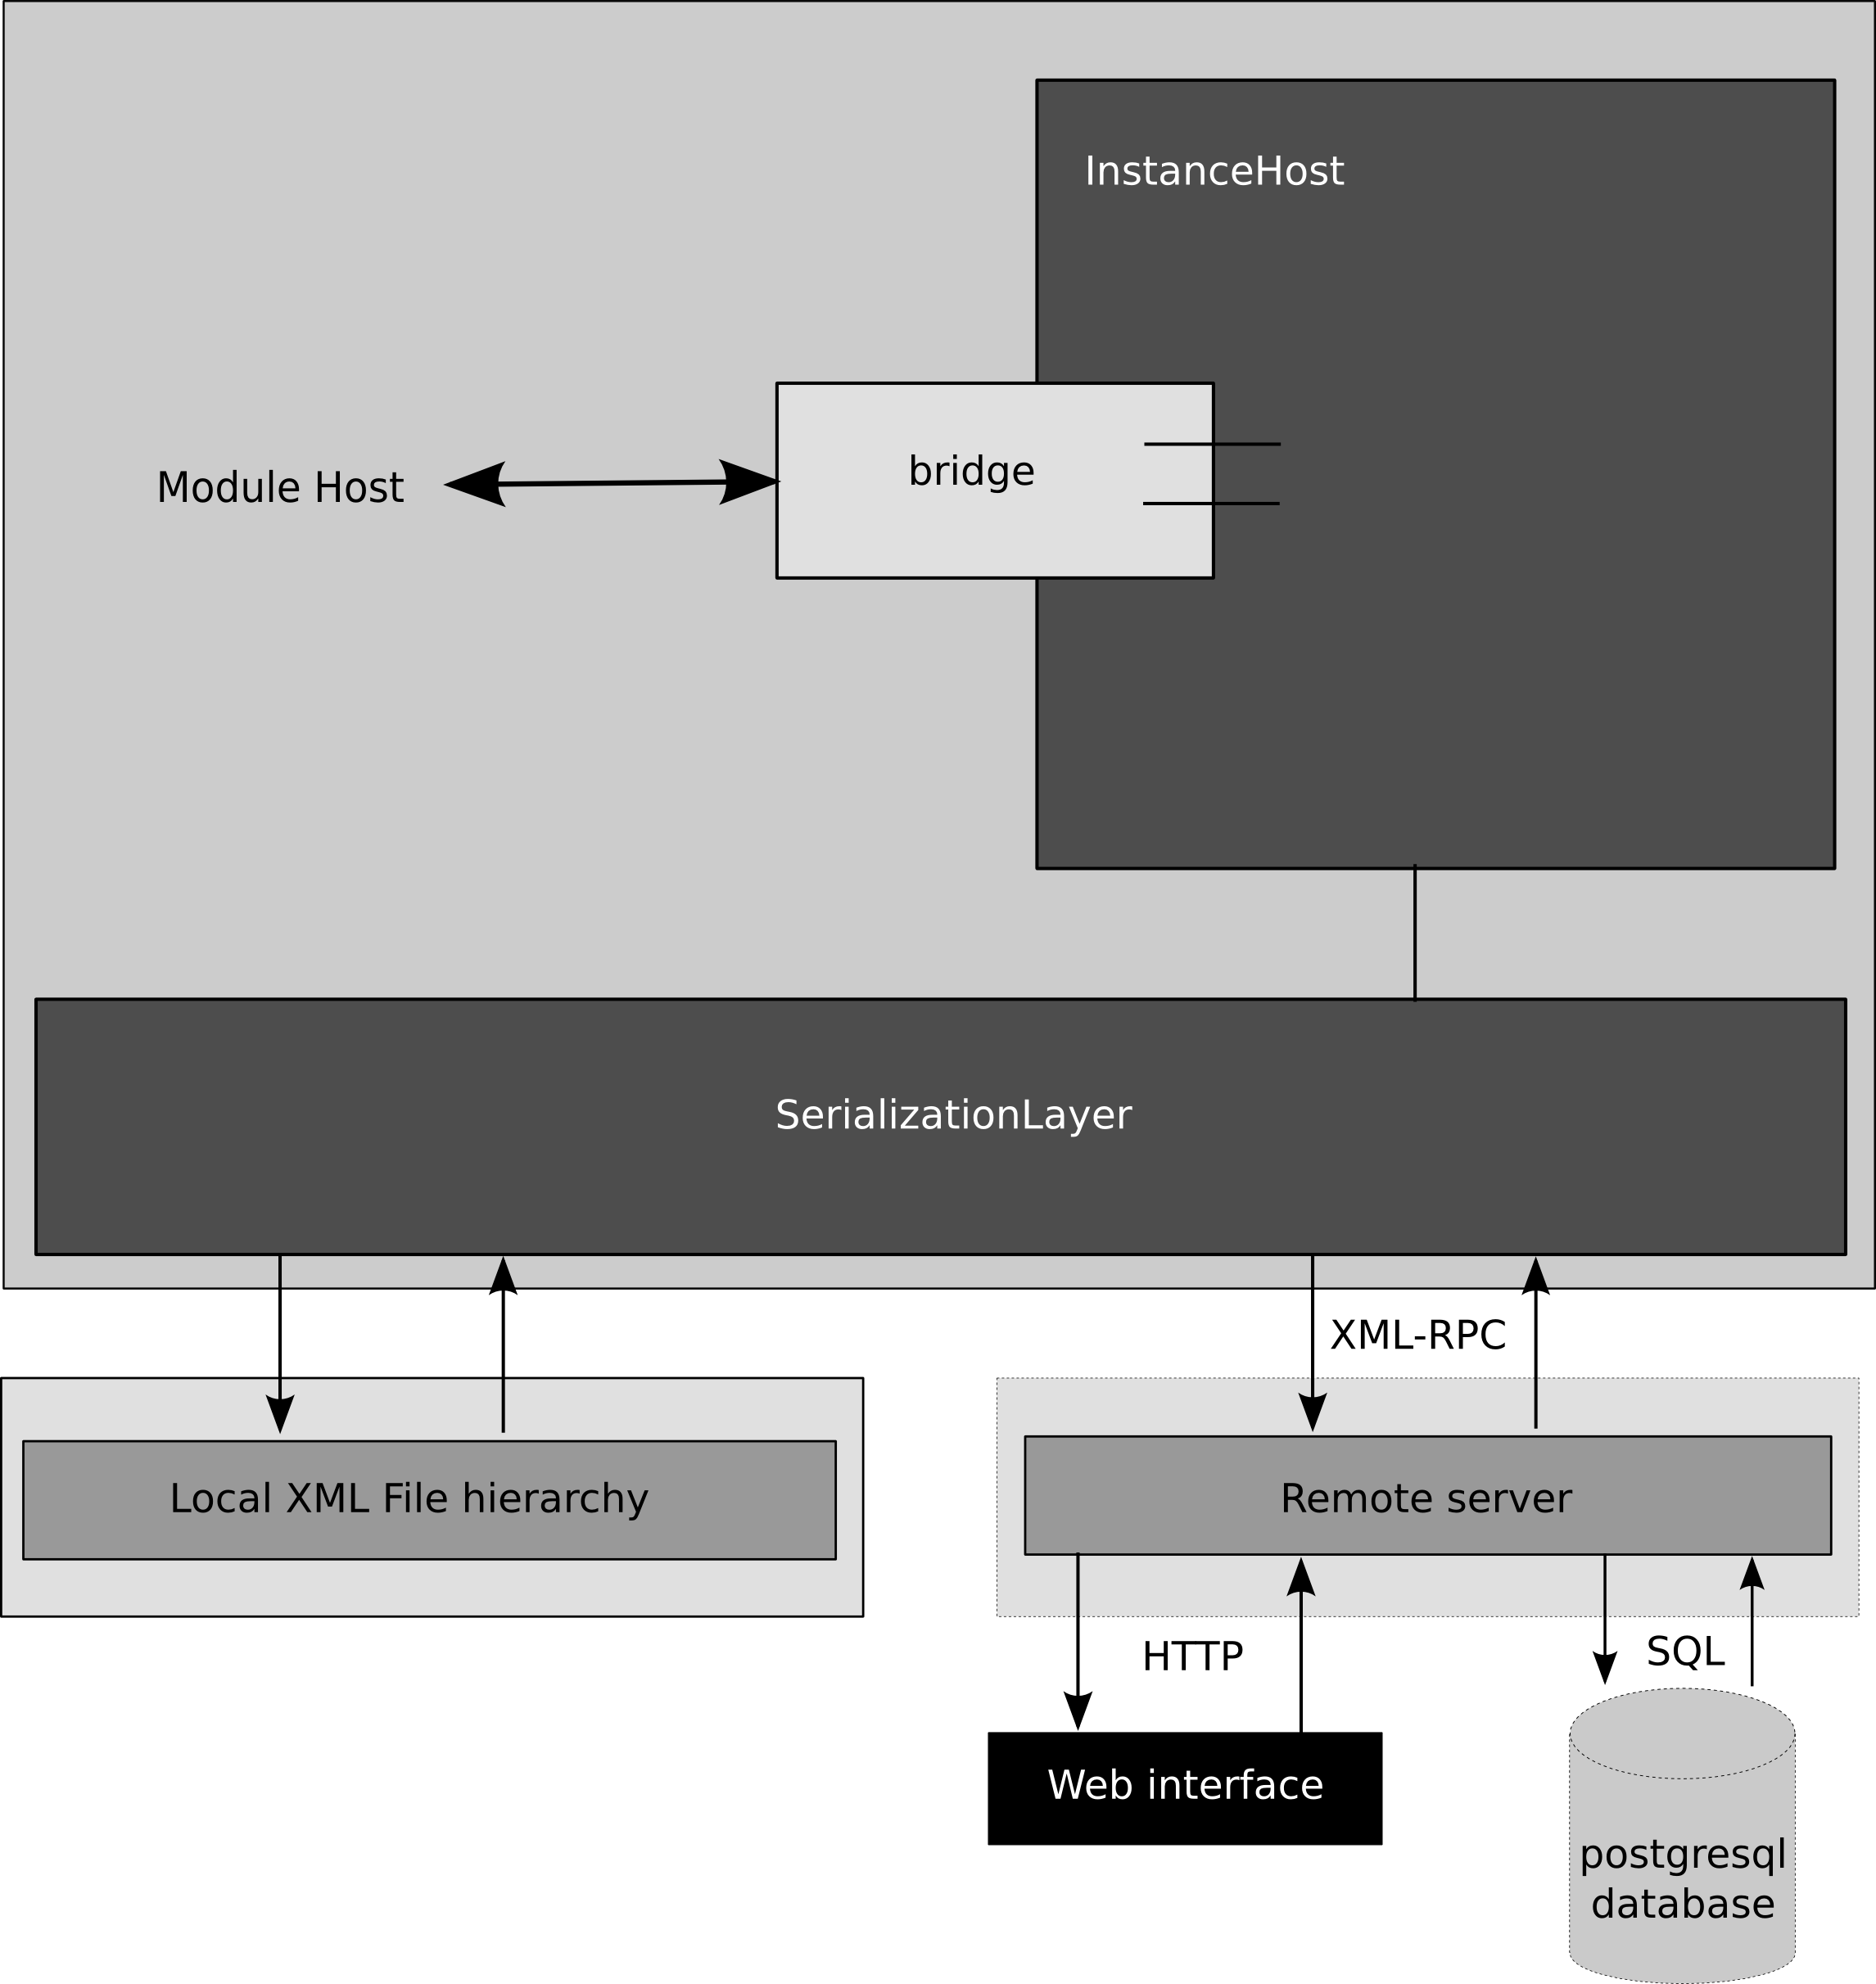
\includegraphics[width=\columnwidth]{img/library_model_small}}}
\caption{A model of the parts constituting libIntegra and how the library interfaces with other parts of the system.}
\label{fig:model}
\end{figure}

\subsection{Module host}\label{subsec:module_host}

The module host is any software that hosts Integra modules: it is not part of libIntegra. Typically, a module host will be dynamically linked to libIntegra at compile time. At run time the module host can make direct calls to functions in the instance host and also make use of the Instance host OSC interface. Typically the OSC interface is used for communication with modules or hosts that are running in a different program or operating system process. Communication from the Instance host to the module host and modules is always achieved through the 'bridge'.

It is also possible for the module host to be a standalone application that doesn't link to libIntegra. In this case the bridge will usually use a network-based protocol such as OSC to communicate with the module host. A Unix pipe or socket is another possibility for this type of setup.

\subsection{Inter-library communication}\label{subsec:interlib}

An arbitrary number of libIntegra instances may be running on the same computer or on any number of networked computers. Each libIntegra instance can be running in a new instance of a common module host, or a completely different module host. A single computer
setup is shown in Figure \ref{fig:model}. 

When multiple libIntegra instances are used, only one (the master), can make use of the serialization layer to load and save Integra module instance data and collections. This is to prevent several versions of the same collection being opened by different library instances, and becoming unsynchronised. If the user or developer knows that the serialization layer will not be required, the library can be compiled without it.

The Instance host contains mechanisms for inter-library communication and auto-discovery. This is mostly achieved through OSC messaging, and facilitates the loading of Integra collections across several module hosts, with transparent state saving.


\section{Conclusion}\label{sec:conclusion}

We have outlined a robust, cross-platform, software-in\-dependent means of storing and loading module data. In addition we have discussed the facilities that the Integra library provides for loading, saving, instantiating and managing modules and collections of modules. The next stage in our work will entail a phase of alpha and beta testing, both internally and with our end-users. The aim of the Integra project is to improve the usability of software for working with live electronics, and to provide a mechanism for the sustainability of the musical works it is used to create. libIntegra should ultimately provide a foundation for this.

%%% Local Variables: 
%%% mode: latex
%%% TeX-master: "../IntegraICMC"
%%% End: 


% \begin{appendices}
%   \chapter{Csound orchestra for \emph{etherSound}}
%   \label{sec:csound-orch-ethers}
%   \input{../../../etherSound/svn/ethsnd/branches/dissertation/include/etherSound-appendix}
% \end{appendices}

\chapter*{\bibname}

\bibliography{bibliography}
\bibliographystyle{newapa}

\end{document}
%%% Local Variables: 
%%% mode: latex
%%% TeX-master: t
%%% End: 
